\documentclass[10pt,a4paper,titlepage]{article}
\usepackage[T1]{fontenc}
\usepackage{graphicx}
\usepackage{amssymb}
\usepackage{hyperref}
\usepackage{float}
\title{Introducción de Linux}
\author{Angel Cruz Olvera}
\begin{document}
	\maketitle
	
	\section*{UNIX}	
	Fue construido en 1969 por un equipo de desarrolladores de los laboratorios Bell en AT\&T Dennis Ritchie, Ken Thompson, Douglas Mcllroy y Joe Osanna. Su nombre original seria UNICS que tiene como significado Uniplexed Information and Computing System. 
	\\
	\\
	Este sistema es de código abierto, lo que el desarrollo y actualización es contribución de los usuarios. Este ademas, es portable, multitarea y multiusuario. UNIX tiene dos componentes principales: la shell y el kernel.
	
	\begin{figure}[H]
		\centering
		
\includegraphics[width=0.5\linewidth]{"./images/unix.png"}
		\caption{Logotipo de sistema operativo UNIX}
		\label{fig:logo-UNIX}
	\end{figure}
	
	
	\section*{GNU}
	Es un sistema operativo de software libre, el cual consiste en paquetes desarrollado por el proyecto GNU, es decir programas publicados específicamente para el proyecto. Inicio en 1984 por Richard Stallman, su nombre es un acrónimo recursivo de GNU No es UNIX. Posteriormente en 1990, se desarrollo GNU Hurd como kernel propio del proyecto.
	
	\begin{figure}[H]
		\centering
		
\includegraphics[width=0.5\linewidth]{"./images/gnu.png"}
		\caption{Logotipo del proyecto GNU.}
		\label{fig:logoGNU}
	\end{figure}
	
	\section*{Linux}
	Creado por Linus Torvalds en 1991, siguiendo el concepto de código abierto basado en UNIX. Se compone de varias partes, siendo el kernel el principal de ellos, puesto que es capaz de gestionar los recursos y permite comunicar el hardware y software del equipo.
	
	\begin{figure}[H]
		\centering
		
\includegraphics[width=0.5\linewidth]{"./images/linux.png"}
		\caption{Logotipo de sistema operativo Linux.}
		\label{fig:logoLinux}
	\end{figure}
	
	\subsection*{Arquitectura}
	La arquitectura de este sistema operativo se llama GNU/Linux, principalmente se divide en dos secciones el espacio del kernel y el espacio de usuario. Cada uno tiene partes diferentes, que ha continuación se enuncian.
	
	\begin{figure}[H]
		\centering
		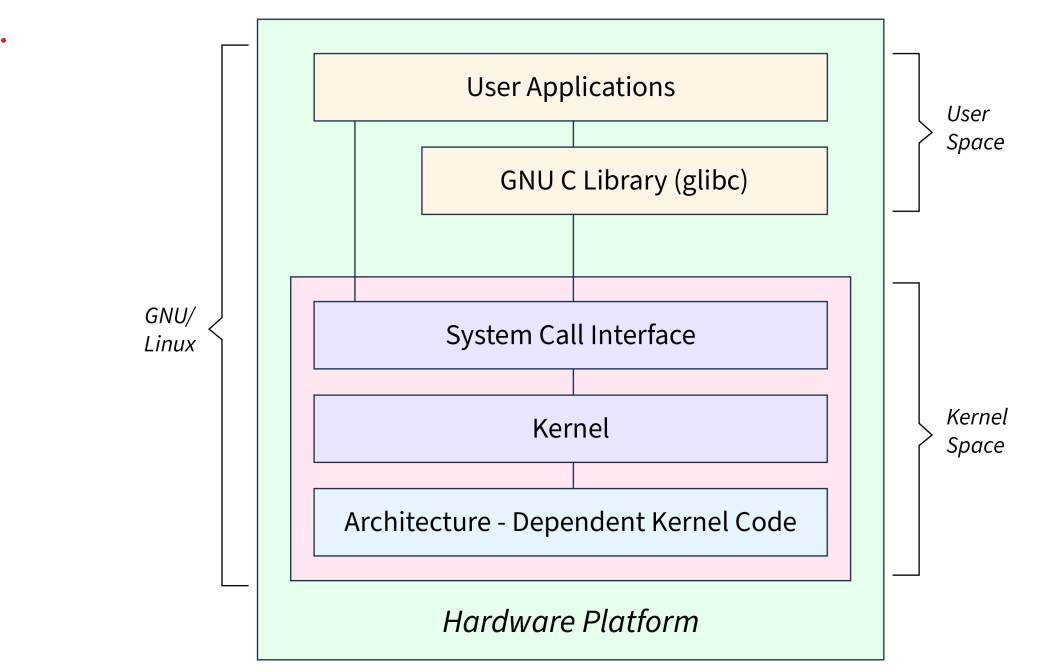
\includegraphics[width=0.9\linewidth]{"./images/arquitectura.png"}
		\caption{Esquema de la arquitectura del sistema GNU/Linux.}
		\label{fig:arquitectura}
	\end{figure}
	
	\subsubsection*{Espacio del kernel}
	
	\emph{Kernel:} es el programa central del sistema, inicia por el boot loader que es el encargado de las interacciones basicas del hardware con el sistema, ya sean tareas de lectura y escritura en disco duro, memoria RAM, controlares de dispositivos, asi como proporcionar un entorno virtual para iniciar las aplicaciones.
	\\
	\\
	\emph{Subsistemas:} son los programas que vienen instalados de manera predeterminada en el sistema, que se encargan de gestionar el acceso remoto, tener un bus central de mensajes/notificaciones y ejecutan acciones basadas en eventos de hardware o red.
	\\
	\\
	\emph{Herramienta de linea de comandos:} son programas pequeños que se ejecutan dentro de la linea de comandos o emulador de terminal, son capaces de editar texto, descargar archivos o administración del sistema.
	\\
	\\
	\emph{Inter Process Communication:} se encarga de tener una comunicación entre el kernel y las aplicaciones, por medio de un segmento compartido de memoria o un pequeño canal de comunicación creado por las aplicaciones para intercambio de datos. Otro método es a través del bus central de mensajes donde hay un intercambio de mensajes para comunicar todo el sistema. 
	
	\subsubsection*{Espacio del usuario}
	\emph{Librerías GNU:} son programas pequeños que controlar las ventanas, gráficos o lectura/escritura de las aplicaciones. Están desarrolladas en lenguaje C y cada una de ellas puede tener mas librerías para poder ser utilizada.
	\\
	\\
	\emph{Aplicaciones:} son todos aquellos programas finales, con los que el usuario puede interactuar con el sistema. Entre ellos están los navegadores web, editores de texto, reproductores de video o sonido, visualizadores de imágenes/videos, editores de imagen/video, entre muchos otros mas.
	
	\subsection*{¿Qué es una distribución?}
	Son configuraciones del kernel dependiendo de las necesidades de cierta comunidad, donde incluye una amplia gama de software, herramientas GNU, bibliotecas, interfaz grafica y aplicaciones. Cuenta con un administrador de paquetes para instalar, actualizar y eliminar software de manera sencilla. Algunas de las distribuciones mas populares son las siguientes:
	\\
	\\
	\emph{Ubuntu:} la mas popular por su facilidad de uso, documentación y soporte comunitario. Esta basado en Debian, lanzando cada seis meses nuevas versiones. Cuenta con versiones para escritorio, servers y cloud.	
	\begin{figure}[H]
		\centering
		
\includegraphics[width=0.3\linewidth]{"./images/ubuntu.png"}
		\caption{Logotipo distribución Ubuntu.}
		\label{fig:logoUbuntu}
	\end{figure}

	\emph{Linux Mint:} enfocado en brindar una experiencia completa lista para usar al incluir complementos de navegador, codecs multimedia y soporte para reproducción de DVD.	
	\begin{figure}[H]
		\centering
		
\includegraphics[width=0.3\linewidth]{"./images/mint.png"}
		\caption{Logotipo distribución Linux Mint.}
		\label{fig:logoMint}
	\end{figure}
	
	\emph{Fedora:} es patrocinado por Red Hat y es utilizado como distribución para su versión de empresa Red Hat Enterprise Linux. 
	\begin{figure}[H]
		\centering
		
\includegraphics[width=0.2\linewidth]{"./images/fedora.png"}
		\caption{Logotipo distribución Fedora.}
		\label{fig:logoFedora}
	\end{figure}
	
	\emph{Debian:} es una de las mas antiguas, estable, seguridad y amplios repositorios de software. Utiliza una amplia gama de arquitecturas y ofrece más $59,000$ paquetes de software, ademas de utilizar la gestión de paquetes con APT y su formato con extensión deb.
	\begin{figure}[H]
		\centering
		
\includegraphics[width=0.3\linewidth]{"./images/debian.png"}
		\caption{Logotipo distribución Debian.}
		\label{fig:logoDebian}
	\end{figure}
	
	\emph{Arch Linux:} dirigido a usuarios mas experimentados, siguiendo un modelo de lanzamiento continuo ofreciendo las ultimas versiones manteniendo la simplicidad y personalización. Utiliza pacman como administrador de paquetes y es conocido por una documentación completa y detallada.
	\begin{figure}[H]
		\centering
		
\includegraphics[width=0.3\linewidth]{"./images/arch.png"}
		\caption{Logotipo distribución Arch Linux.}
		\label{fig:logoArch}
	\end{figure}
	
	\subsection*{Comparativa}
	
	\section*{Comandos basicos}
	
	\section*{Administración}
	
	\section*{Networking}
	
	\section*{Referencias}
	FYCGROUP. UNIX: La simplicidad del ingenio, fyccorp.com consultado el 17 de agosto de 2025, recuperado de https://fyccorp.com/unix-la-simplicidad-del-ingenio/	
	\\
	\\
	GNU. ¿Qué es GNU?, www.gnu.org, consultado el 17 de agosto de 2025, recuperado de https://www.gnu.org/home.es.html
	\\
	\\
	Floriano, J.(2024). ¿Qué es el sistema Linux y cuáles son sus ventajas?, BlogSEAS, consultado el 17 de agosto de 2025, recuperado de https://www.seas.es/blog/informatica/que-es-el-sistema-linux-y-cuales-son-sus-ventajas/
	\\
	\\
	Denisse. (2016). Una mirada dentro del núcleo de Linux, lignux.com, consultado el 18 de agosto de 2025, recuperado de https://lignux.com/una-mirada-dentro-del-nucleo-linux/
	\\
	\\
	Spasojevic, A. (2024). ¿Qué es una distribución de Linux?, phoenixnap.mx, consultado el 18 de agosto de 2025, recuperado de https://phoenixnap.mx/glosario/que-es-una-distribucion-de-linux
	
\end{document}